\documentclass[10pt,aps,onecolumn,superscriptaddress]{revtex4-2}

\usepackage[T1]{fontenc}
\usepackage[utf8]{inputenc}
\usepackage[english]{babel}

\usepackage{amsfonts,amsbsy,amssymb,amsmath}
\usepackage{graphicx,float}
\usepackage{hyperref}
\hypersetup{
    colorlinks=true,
    linkcolor=blue,
    filecolor=magenta,      
    urlcolor=cyan,
}

\graphicspath{{notebooks/figures/}}

\bibliographystyle{apsrev4-2}

\begin{document}

\title{Chemical Reaction Dynamics on the Cirque Potential Energy Surface}

\author{Broncio Aguilar Sanjuan}
\email{broncio.aguilarsanjuan@bristol.ac.uk}
\affiliation{School of Mathematics, University of Bristol, \\ Fry Building, Woodland Road, Bristol, BS8 1UG, United Kingdom.}

\author{V\'ictor J. Garc\'ia-Garrido}
\email{vjose.garcia@uah.es}
\affiliation{Departamento de F\'isica y Matem\'aticas, Universidad de Alcal\'a, \\ Alcal\'a de Henares, 28871, Spain.}

\author{Francisco Gonz\'alez Montoya}
\email{fg16704@bristol.ac.uk}
\affiliation{School of Mathematics, University of Bristol, \\ Fry Building, Woodland Road, Bristol, BS8 1UG, United Kingdom.}

\author{Stephen Wiggins}
\email{s.wiggins@bristol.ac.uk}
\affiliation{School of Mathematics, University of Bristol, \\ Fry Building, Woodland Road, Bristol, BS8 1UG, United Kingdom.}


\date{\today}


\begin{abstract}

In this paper we explore the bifurcation scenario when the energy is increased.

% Energy before the threshold E < 0,  Closed system
% Energies corresponding to the bifurcation of the periodic orbits type I , II , III, Open system
%% Conjecture E_I > E_II > E_III

\end{abstract}

\maketitle

\noindent\textbf{Keywords:} Phase space structure, Chemical reaction dynamics, Roaming, Lagrangian descriptors, 

\section{Introduction}


Single VdW potential \cite{Soley2018}. It models the long-range interaction describing dipole-dipole attraction between neutral molecules/atoms
\begin{equation}
    V(r) = -\dfrac{C}{(\beta r^2 + \alpha)^3}
    \label{eq:vdw-single}
\end{equation}
Potential is parametrized to remove singularity from origin, $r = 0$. We have that $C$ is the van der Waals dispersion coefficient, and $\alpha$ and $\beta$  - the characteristic length parameter - are positive parametrization constants. The potential's minimum is located at position $r = r_e = 0$, with energy 
\begin{equation}
    V\left(r_e \right) = - \dfrac{C}{\alpha^3}
\end{equation}
Note that when $r \longrightarrow + \infty$, the leading order form of the potential is
\begin{equation}
    V(r \longrightarrow +\infty) \sim - \frac{C}{r^6 \beta^3}
\end{equation}
Since the potential only depends on the radial distance from the origin, it is axially symmetric when considered as a function in the 2D plane.

An alternative way that we can use to write the model, so that its parameters have a geometrical interpretation regarding the shape of the potential energy function is the following. Consider the function:
\begin{equation}
W(\mathbf{r}) = - \dfrac{W_0}{\left(\dfrac{1}{k^2} |\mathbf{r}|^2 + 1\right)^3} = - \dfrac{W_0 k^6}{\left( |\mathbf{r}|^2 + k^2\right)^3}
\label{eq:heller_pes}
\end{equation}
where $\mathbf{r} = (x,y)$ is the position vector. It is straightforward to show that $W_0$ represents the depth of the potential well located at the origin with respect to the dissociation energy, which is given by:
\begin{equation}
W_{\infty} = \lim_{|\mathbf{r}| \to \infty} W(\mathbf{r}) = 0
\end{equation}
Moreover, the parameter $k$ determines the half-width of the well as measured at the energy level corresponding to one eighth the energy of the minimum at the bottom of the well. We can shift the PES in Eq. \eqref{eq:heller_pes} to any point $\mathbf{r}_0 = (x_0,y_0)$ in configuration space by considering:
\begin{equation}
W_{\mathbf{r}_0}(\mathbf{r}) = W(\mathbf{r} - \mathbf{r}_0) = - \dfrac{W_0 k^6}{\left( |\mathbf{r} - \mathbf{r}_0|^2 + k^2\right)^3} = - \dfrac{W_0 k^6}{\left(\left(x-x_0\right)^2 + \left(y-y_0\right)^2 + k^2\right)^3}
\end{equation}
and the double van der Waals PES used to model the Cirque energy landscape can be easily constructed by means of choosing two points on the $x$-axis separated the same distance $d$ from the origin, that is, $\mathbf{r}_{1,2} = (\pm d,0)$, and superposing their potentials so that:
\begin{equation}
V(\mathbf{r}) \equiv V(x,y) =  W_{\mathbf{r}_1}(\mathbf{r}) + W_{\mathbf{r}_2}(\mathbf{r})
= - W_0 k^6 \left[\dfrac{1}{\left(\left(x - d\right)^2 + y^2 + k^2\right)^3} + \dfrac{1}{\left(\left(x + d\right)^2 + y^2 + k^2\right)^3} \right]
\end{equation}


\begin{figure}[htbp]
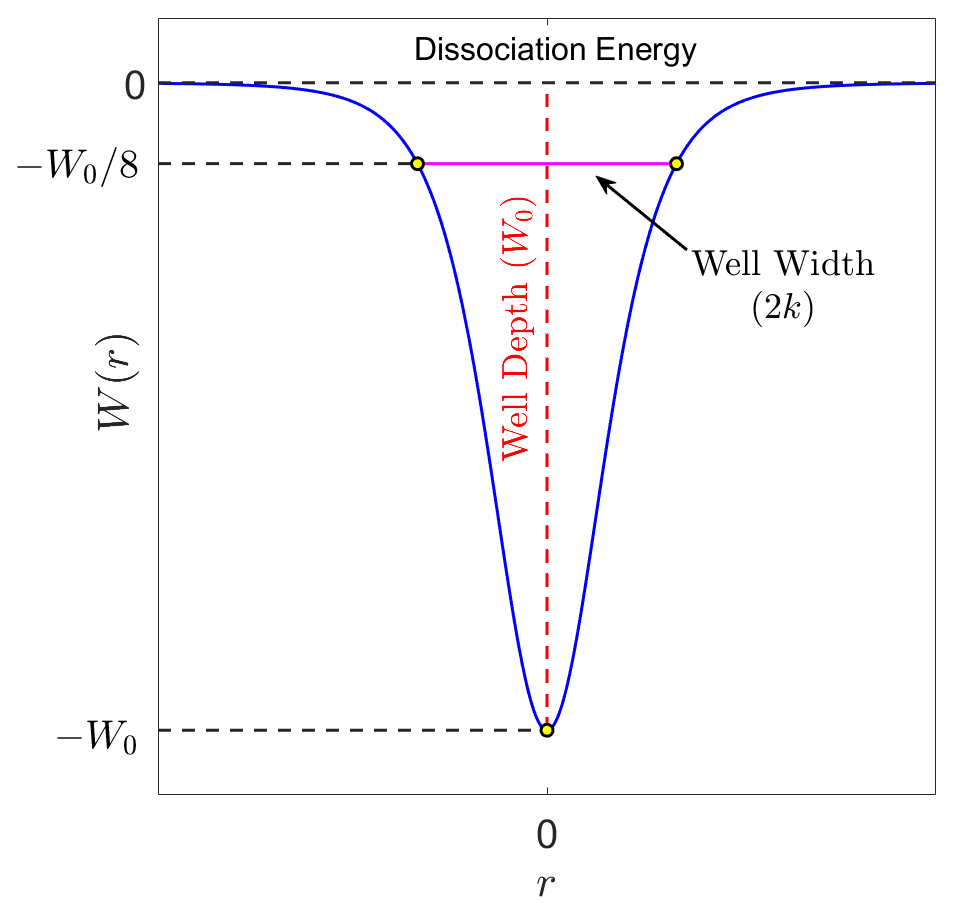
\includegraphics[scale=0.35]{heller_potFunc_new2.png}
\caption{Geometrical interpretation of the parameters that determine the shape of the potential energy function in Eq. \eqref{eq:heller_pes}.}
\label{fig:heller_pes}
\end{figure}





\section{Double van der Waals Potential}

To construct a double-well potential using the formula \eqref{eq:vdw-single}, in a similar way to the double Morse potential \cite{GonzalezMontoya2020}, we need first, to express the potential in 2D cartesian coordinates and then, vary the separation between the minima of two overlapped potentials along the x-axis

\textbf{First Proposal} using potential \eqref{eq:vdw-single}

Displace potentials radially by a common distance $d$ from the origin in the $x$-axis direction
\begin{equation}
    V(x, y) = -C \left[ \dfrac{1}{\left(\beta\left[\left(x - d\right)^2 + y^2\right] + \alpha\right)^3} + \dfrac{1}{\left(\beta\left[\left(x + d\right)^2 + y^2\right] + \alpha\right)^3} \right]
    \label{eq:vdw-double}
\end{equation}

To plot the potential you can try the values $C = 1/2$, $\alpha = 1$, $\beta = 1/8$ and $d = 1$. We have to understand what is the effect on the topography of the PES by changing any of the parameters that appear in the definition of $V(x,y)$

\begin{figure}[htbp]
    A)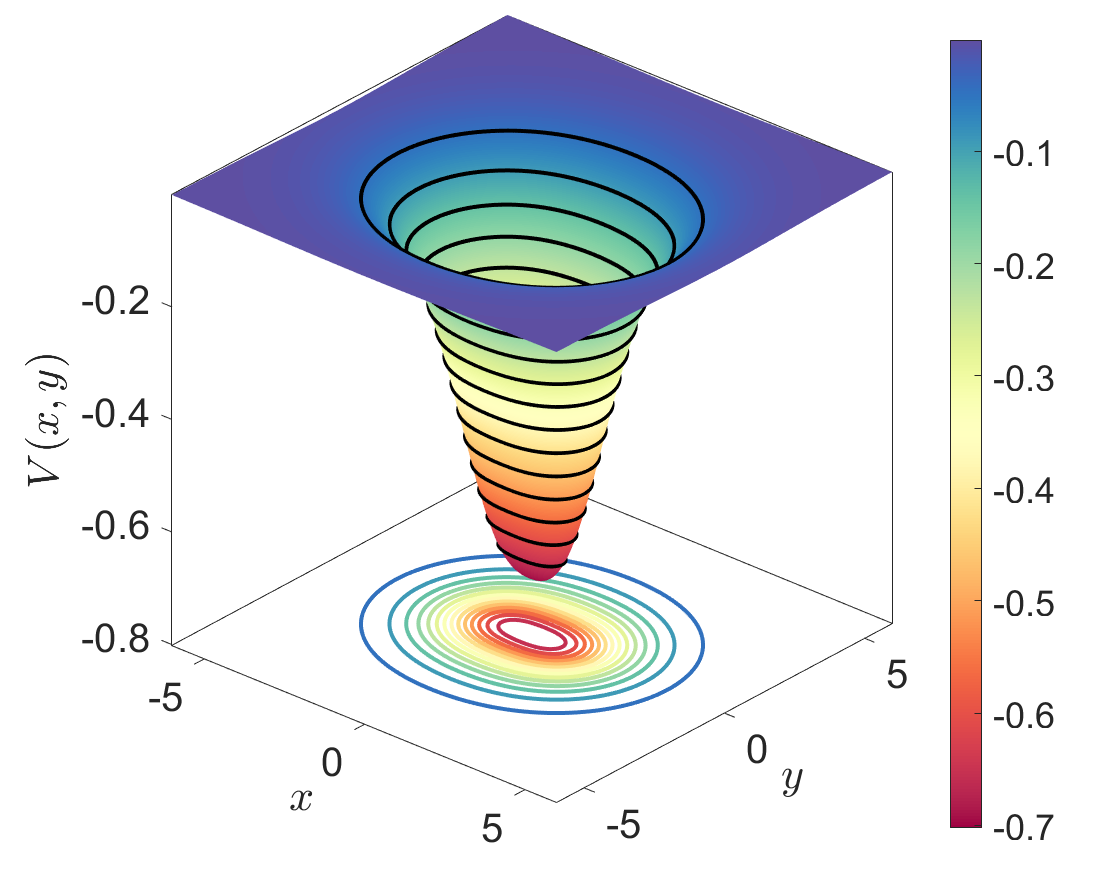
\includegraphics[scale=0.26]{CirquePES_c_1div2_a_1_b_1div8_d_1.png}
    B)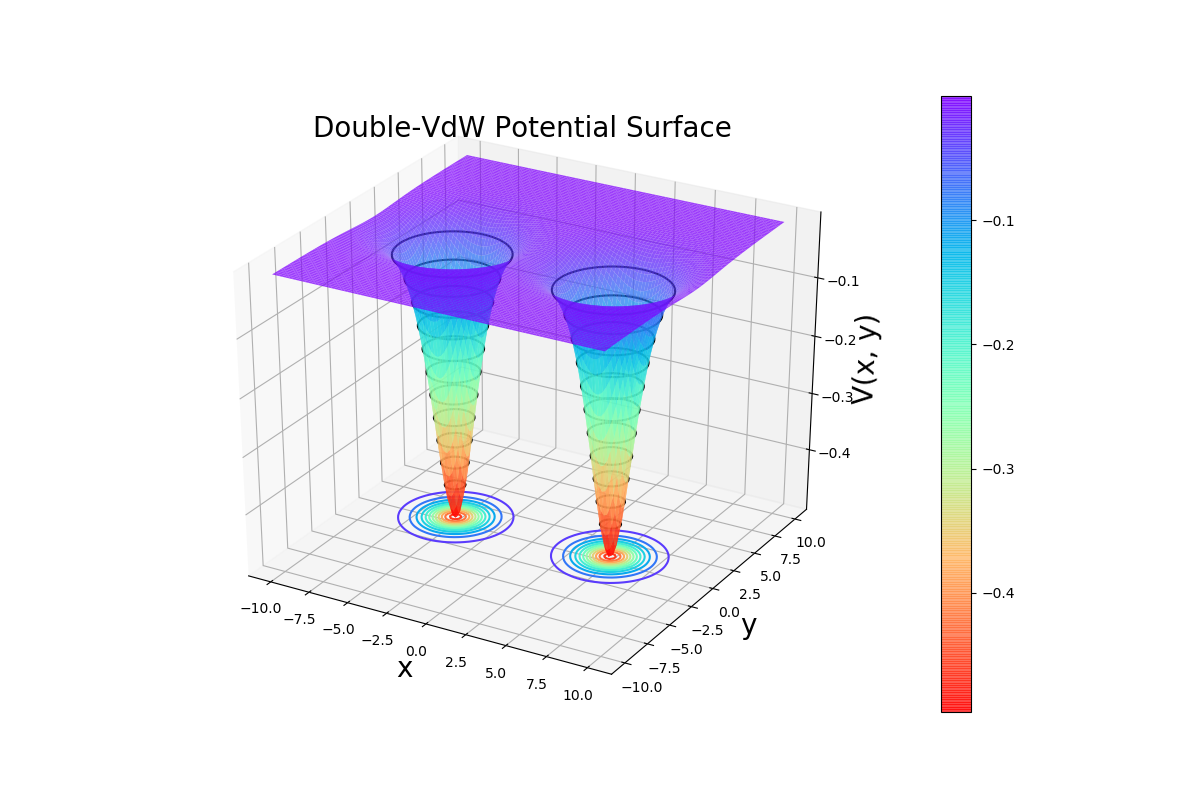
\includegraphics[scale=0.32]{double-vdw_surface.png}
    \caption{Double van der Waals PES in Eq. \eqref{eq:vdw-single} for the model parameters: A) $C = 1/2$, $\alpha = 1$, $\beta = 1/8$ and $d = 1$; B) $C = 1/2$, $\alpha = 1$, $\beta = 1/8$, and $d = 5$.}
    \label{fig:vdw-single_surface}
\end{figure}

The two degrees-of-freedom Hamiltonian for the Cirque potential energy surface is defined as the classical sum of kinetic plus potential energy:
\begin{equation}
H(x,y,p_x,p_y) = \dfrac{p_x^2}{2 m_1} + \dfrac{p_y^2}{2 m_2} + V(x,y)
\label{eq:hamil}
\end{equation}

Hamilton's equations that determine the systems dynamical evolution are given by:
\begin{equation}
    \begin{cases}
    \dot{x} = \dfrac{\partial H}{\partial p_x} = \dfrac{p_x}{m_1} \\[.5cm]
    \dot{y} = \dfrac{\partial H}{\partial p_y} = \dfrac{p_y}{m_2} \\
    \dot{p}_x = - \dfrac{\partial H}{\partial x} = - \dfrac{\partial V}{\partial x} = - 6 \, \beta \, C \left[\dfrac{x - d}{\left(\beta\left[\left(x - d\right)^2 + y^2\right] + \alpha\right)^4} + \dfrac{x + d}{\left(\beta\left[\left(x + d\right)^2 + y^2\right] + \alpha\right)^4}\right] \\[.7cm]
    \dot{p}_y = - \dfrac{\partial H}{\partial y} = - \dfrac{\partial V}{\partial y} = - 6 \, \beta \, C \, y \left[\dfrac{1}{\left(\beta\left[\left(x - d\right)^2 + y^2\right] + \alpha\right)^4} + \dfrac{1}{\left(\beta\left[\left(x + d\right)^2 + y^2\right] + \alpha\right)^4}\right]
    \end{cases}
    \label{eq:ham_eq}
\end{equation}
In this work we will consider the situation where both DoF have unit mass, that is $m_1 = m_2 = 1$. The equilibrium points $\mathbf{r}_e = (x_e,y_e,p_{x,e},p_{y,e})$ of the dynamical system given above are contained in configuration space, since $p_{x,e} = p_{y,e} = 0$, and they are also critical points of the PES, that is $\nabla V (x_e,y_e) = \mathbf{0}$. It is straightforward to check that under these conditions, the points have to satisfy:
\begin{equation}
y_e = 0 \quad , \quad \left(x_e - d\right) \left[\beta\left(x_e + d\right)^2 + \alpha\right]^4 + \left(x_e + d\right) \left[\beta\left(x_e - d\right)^2 + \alpha\right]^4 = 0 
\label{eq:eq_pts}
\end{equation}
It is straightforward to show that $x_e = 0$ is always a solution to the equation above, and therefore the origin is always an equilibrium point of Hamilton's equations for this system. Moreover, there is also an equilibrium point located at infinity. Regarding the presence of other equilibria, this depends critically on the model parameters, and if they exist, their coordinates are of the form $\mathbf{r}_e = (x_e(\alpha,\beta,d),0,0,0)$. 

The linear stability of these equilibrium points is determined by the eigenvalues of the Jacobian matrix given by the linearization of Eq. \eqref{eq:ham_eq} about each of the points. In order to construct the Jacobian, we need to compute the second order partial derivatives that characterize the Hessian matrix of the PES:
\begin{equation}
\begin{cases}
\dfrac{\partial^{\,	2} V}{\partial x^2} = 6 \, \beta \, C \left[\dfrac{\beta\left[-7\left(x - d\right)^2 + y^2\right] + \alpha}{\left(\beta\left[\left(x - d\right)^2 + y^2\right] + \alpha\right)^5} + \dfrac{\beta\left[-7\left(x + d\right)^2 + y^2\right] + \alpha}{\left(\beta\left[\left(x + d\right)^2 + y^2\right] + \alpha\right)^5} \right] \\[.8cm]

\dfrac{\partial^{\,	2} V}{\partial y^2} = 6 \, \beta \, C \left[\dfrac{\beta\left[\left(x - d\right)^2 - 7 y^2\right] + \alpha}{\left(\beta\left[\left(x - d\right)^2 + y^2\right] + \alpha\right)^5} + \dfrac{\beta\left[\left(x + d\right)^2 - 7y^2\right] + \alpha}{\left(\beta\left[\left(x + d\right)^2 + y^2\right] + \alpha\right)^5} \right] \\[.8cm]

\dfrac{\partial^{\,	2} V}{\partial x \partial y} = - 48 \, \beta^2 \, C \, y \left[\dfrac{x - d}{\left(\beta\left[\left(x - d\right)^2 + y^2\right] + \alpha\right)^5} + \dfrac{x + d}{\left(\beta\left[\left(x + d\right)^2 + y^2\right] + \alpha\right)^5}\right]
\end{cases}
\label{eq:second_pder}
\end{equation}
We take a look now at the Hessian matrix of the PES evaluated at the origin:
\begin{equation}
\text{Hess}_{V}(0,0) = \begin{pmatrix}
\dfrac{\partial^{\,	2} V}{\partial x^2}(0,0) & \dfrac{\partial^{\,	2} V}{\partial x \partial y}(0,0) \\[.4cm]
\dfrac{\partial^{\,	2} V}{\partial y \partial x}(0,0) & \dfrac{\partial^{\, 2} V}{\partial y^2}(0,0)
\end{pmatrix} = \begin{pmatrix}
\dfrac{12 \beta C}{\left(\beta d^2 + \alpha\right)^4} \left[1 - \dfrac{8\beta d^2}{\beta d^2 + \alpha}\right] & 0 \\[.5cm]
0 & \dfrac{12 \beta C}{\left(\beta d^2 + \alpha\right)^4}
\end{pmatrix}
\end{equation}
The linear stability of the origin is characterized by the nature of the eigenvalues of the Jacobian matrix:
\begin{equation}
J(0,0) = \begin{pmatrix}
\mathbb{O}_2 & \mathbb{I}_2 \\[.3cm]
-\text{Hess}_{V}(0,0) & \mathbb{O}_2
\end{pmatrix} = \begin{pmatrix}
0 & 0 & \hspace{.2cm} 1 & \hspace{.5cm} 0 \hspace{.2cm} \\[.4cm]
0 & 0 & \hspace{.2cm} 0 & \hspace{.5cm} 1 \hspace{.2cm} \\[.4cm]
\dfrac{12 \beta C}{\left(\beta d^2 + \alpha\right)^4} \left[\dfrac{8\beta d^2}{\beta d^2 + \alpha} - 1\right] & 0 & \hspace{.2cm} 0 & \hspace{.5cm} 0 \hspace{.2cm} \\[.4cm]
0 & -\dfrac{12 \beta C}{\left(\beta d^2 + \alpha\right)^4} & \hspace{.2cm} 0 & \hspace{.5cm} 0 \hspace{.2cm} 
\end{pmatrix}
\end{equation}
The eigenvalues $\xi$ are given by:
\begin{equation}
\xi_{1,2} = \pm \, \omega \, i \quad,\quad \xi_{3,4} = \pm \, \omega \, \sqrt{\dfrac{8\beta d^2}{\beta d^2 + \alpha} - 1}
 \end{equation}
where we have that:
\begin{equation}
\omega = \dfrac{2 \sqrt{3\beta C}}{\left(\beta d^2 + \alpha\right)^2}
\end{equation}

is the angular frequency of oscillation in the linear approximation. Therefore, the origin is an index-1 saddle equilibrium point when the condition $7\beta d^2 \geq \alpha$ is met. However, for $7\beta d^2 < \alpha$ it turns out into a potential well (a center equilibrium point). This indicates that there is a pitchfork bifurcation taking place in the PES at the origin at the critical relation $7\beta d^2 = \alpha$. We illustrate this behavior below by looking at the value of the potential along the $x$-axis:

\begin{figure}
    \centering
    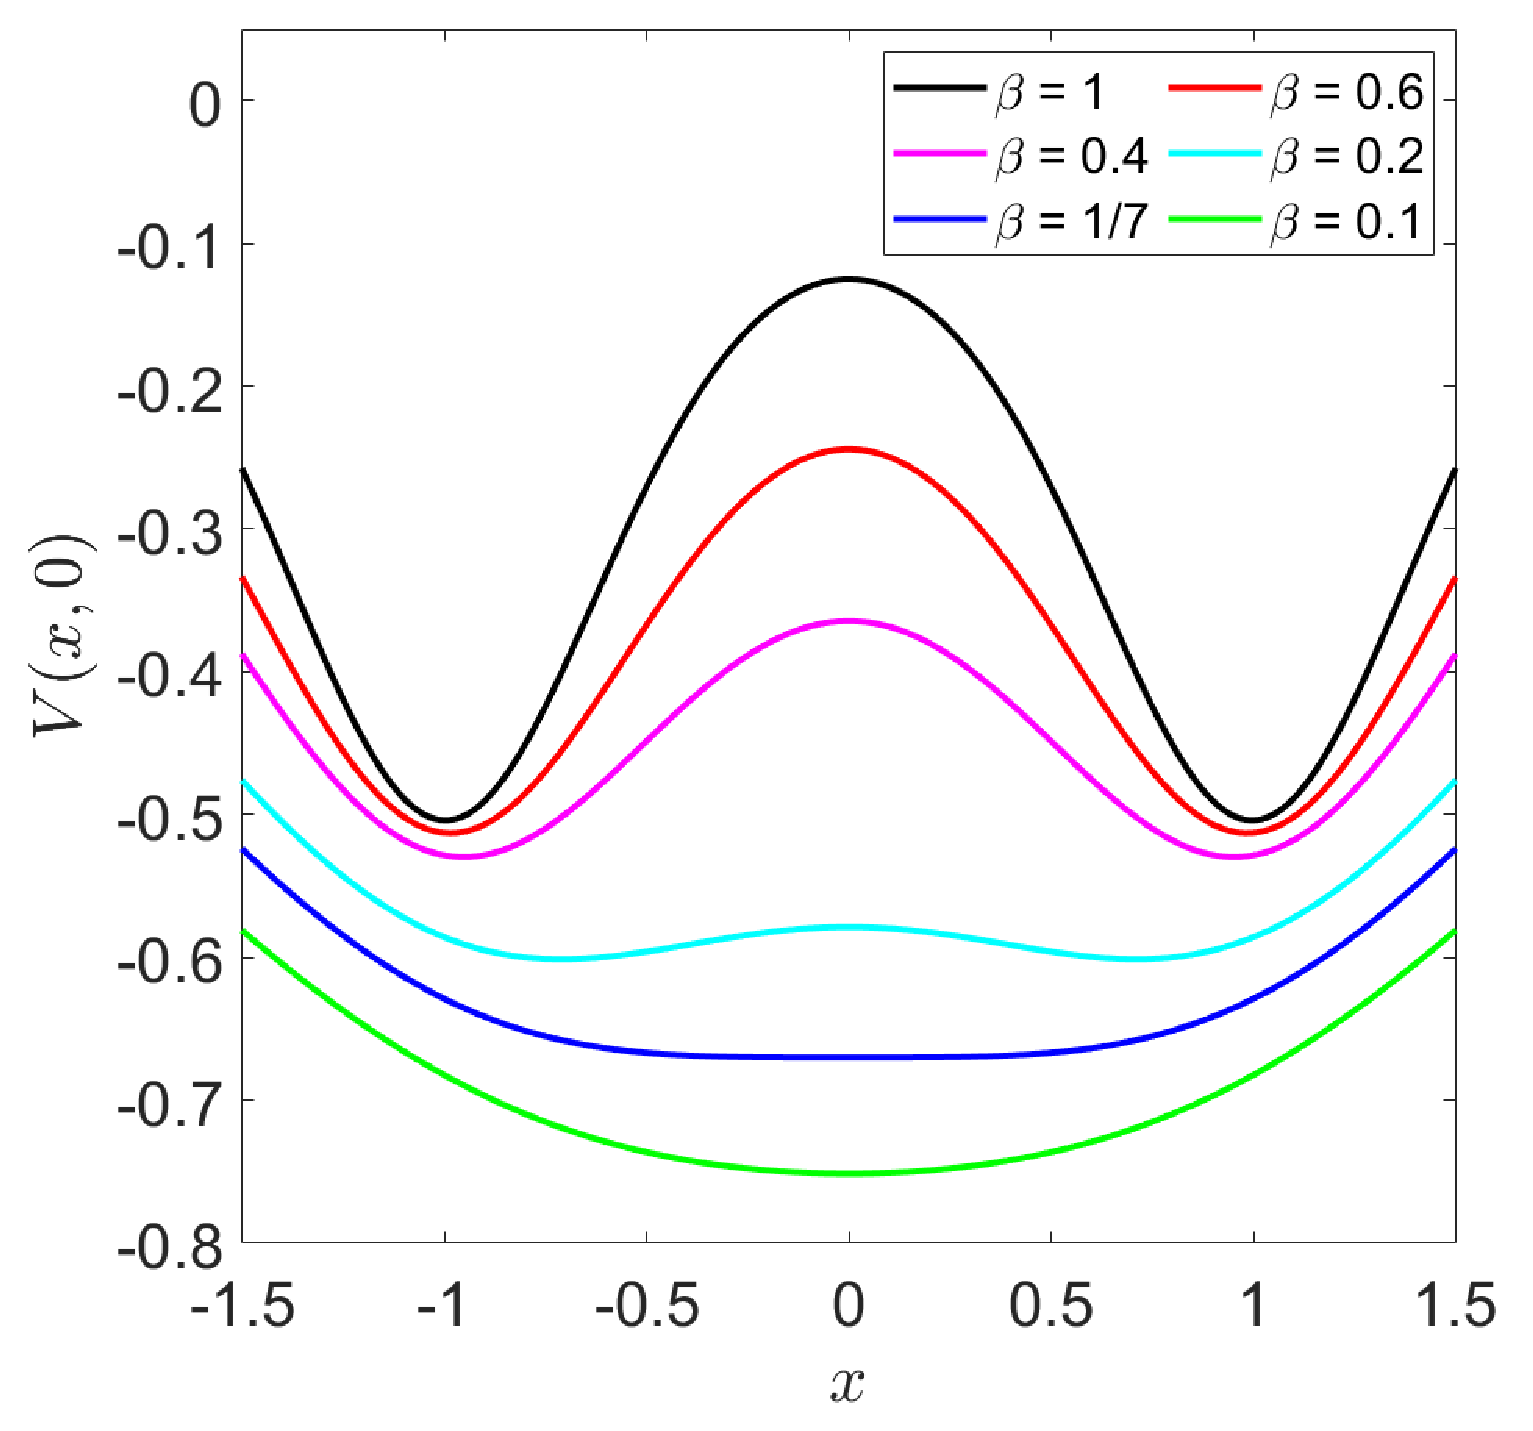
\includegraphics[scale=0.36]{pitcfork_bif_c_1div2_a_1_d_1}
    \caption{}
    \label{fig:pitchfork_bif}
\end{figure}

\section{Results}
\label{sec:results}


\begin{figure}[htbp]
	A)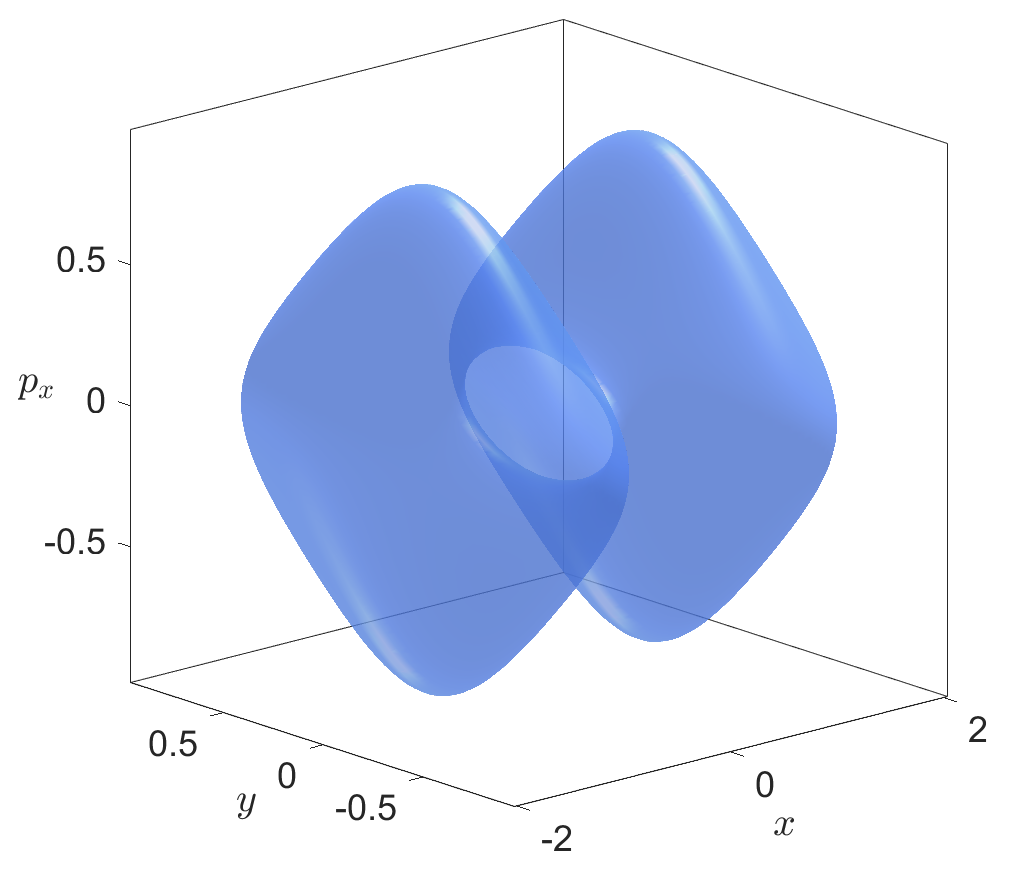
\includegraphics[scale=0.28]{energySurf_H_-01.png}
	B)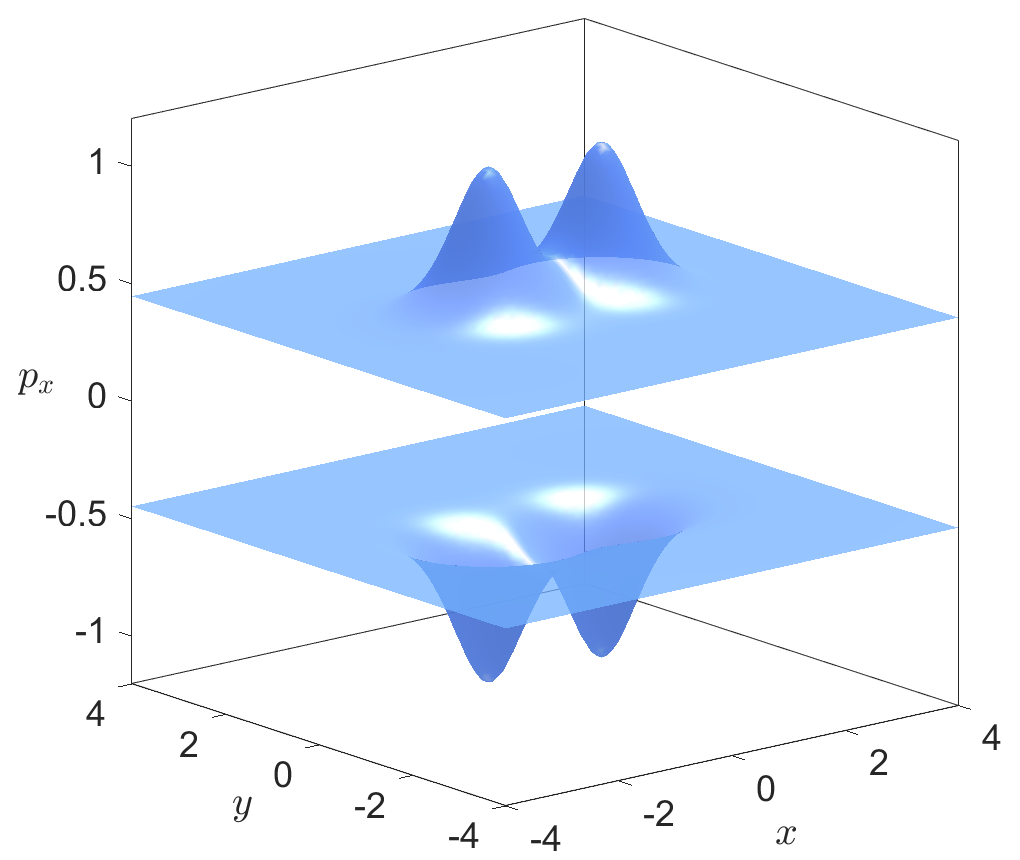
\includegraphics[scale=0.28]{energySurf_H_01.png}
	\caption{$W_0 = 1/2$ and $k = 1$. A) $H_0 = -0.1$; B) $H_0 = 0.1$.}
	\label{fig:vdw-energyHyp}
\end{figure}

\begin{figure}[htbp]
	A)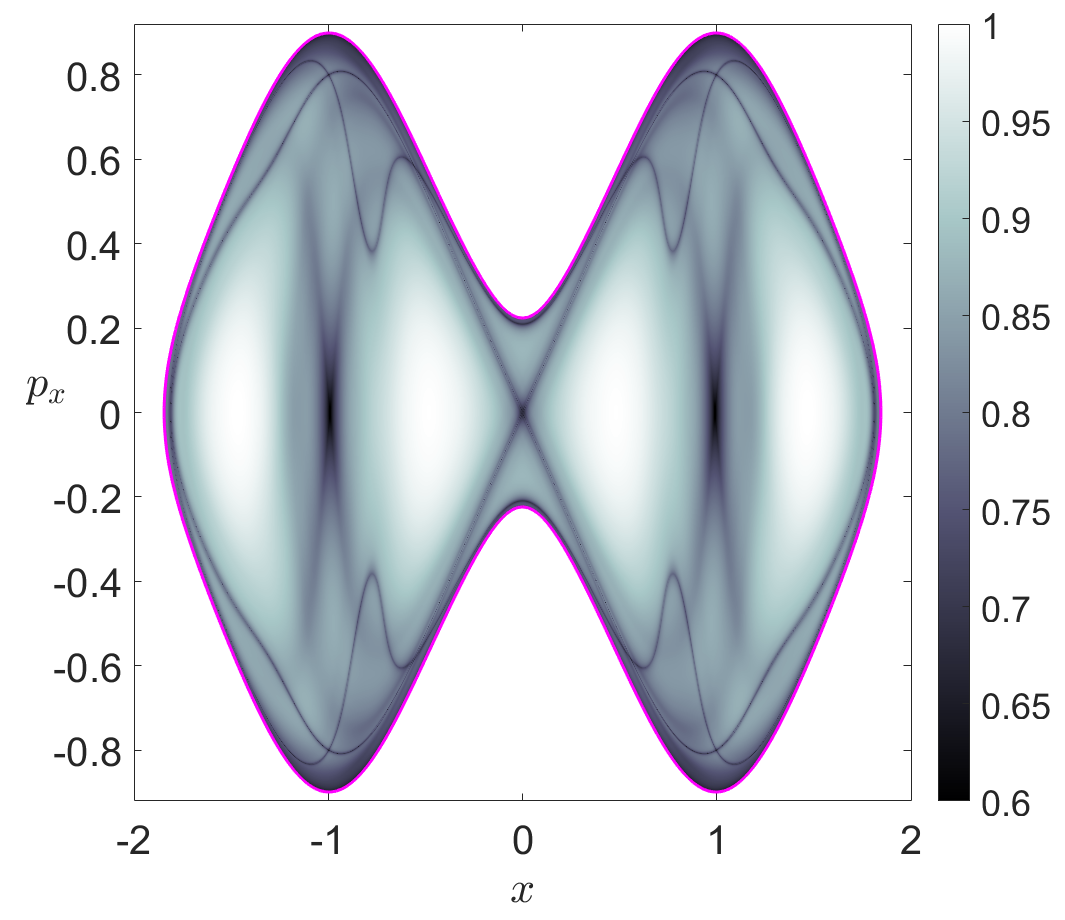
\includegraphics[scale=0.28]{H_-01_LD_tau_12_y_0.png}
	B)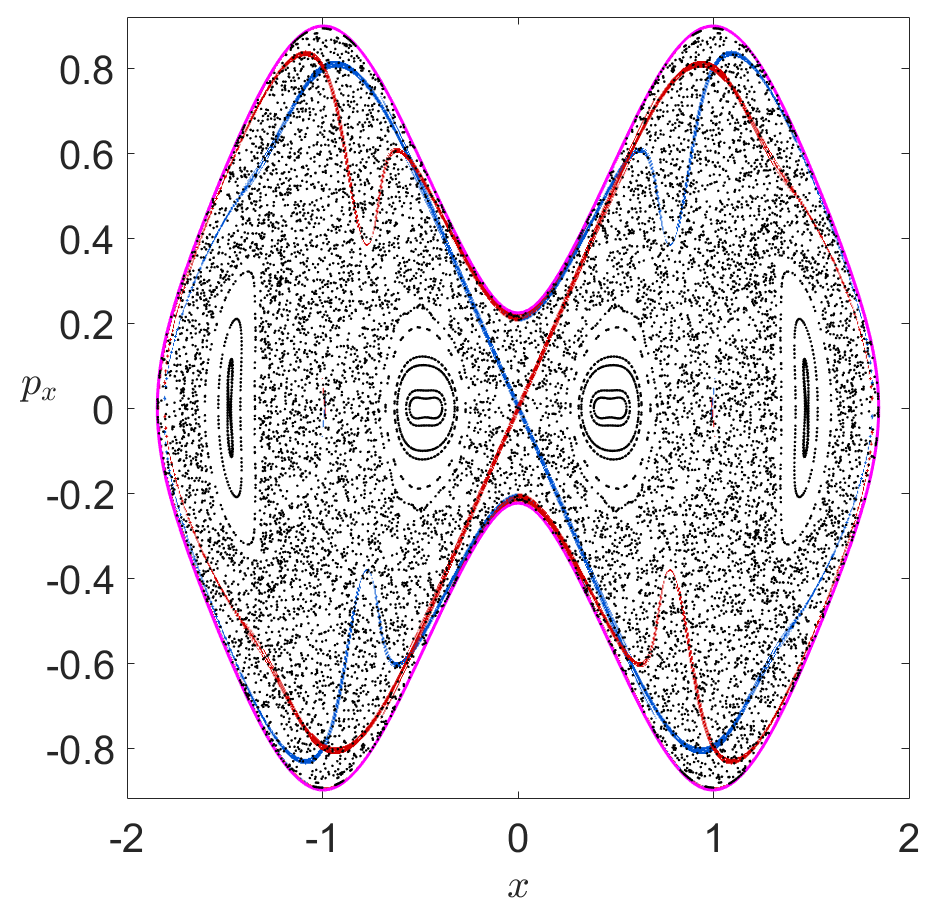
\includegraphics[scale=0.28]{H_-01_mani_tau_12_y_0.png}	
	C)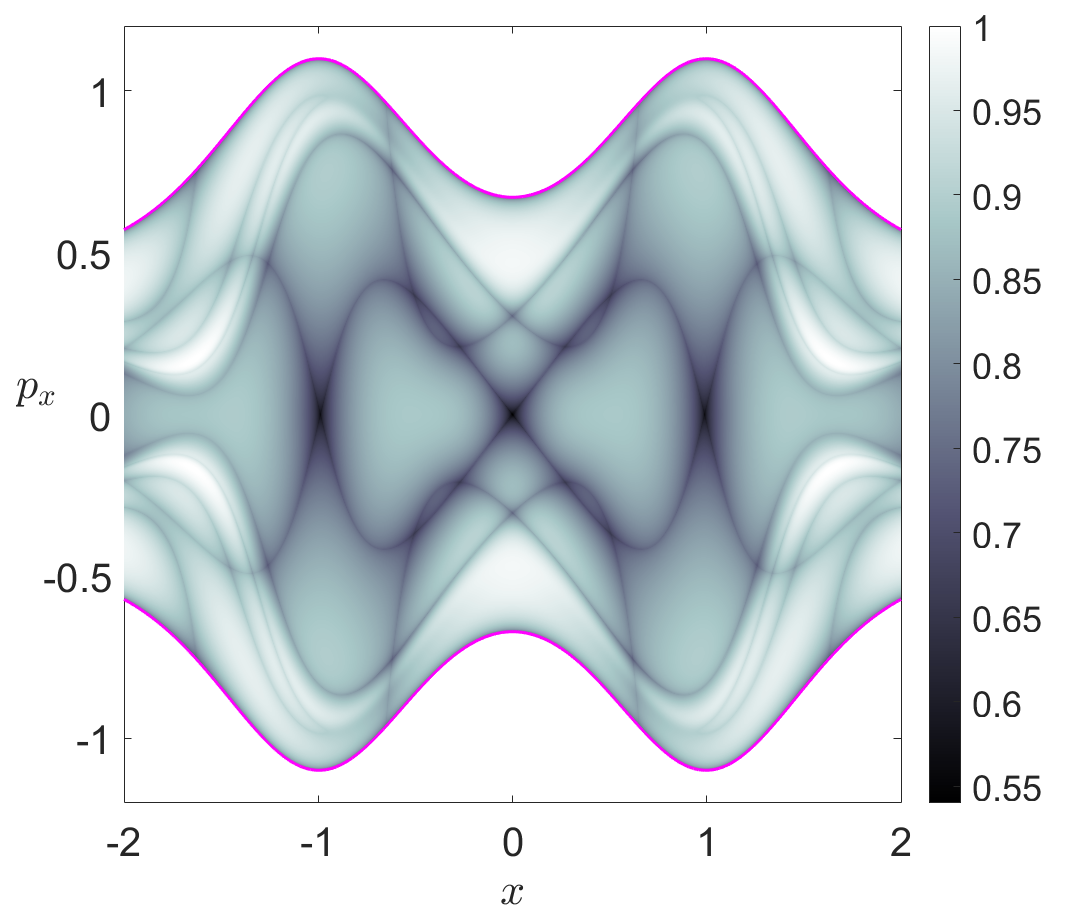
\includegraphics[scale=0.28]{H_01_LD_tau_12_y_0.png}
	D)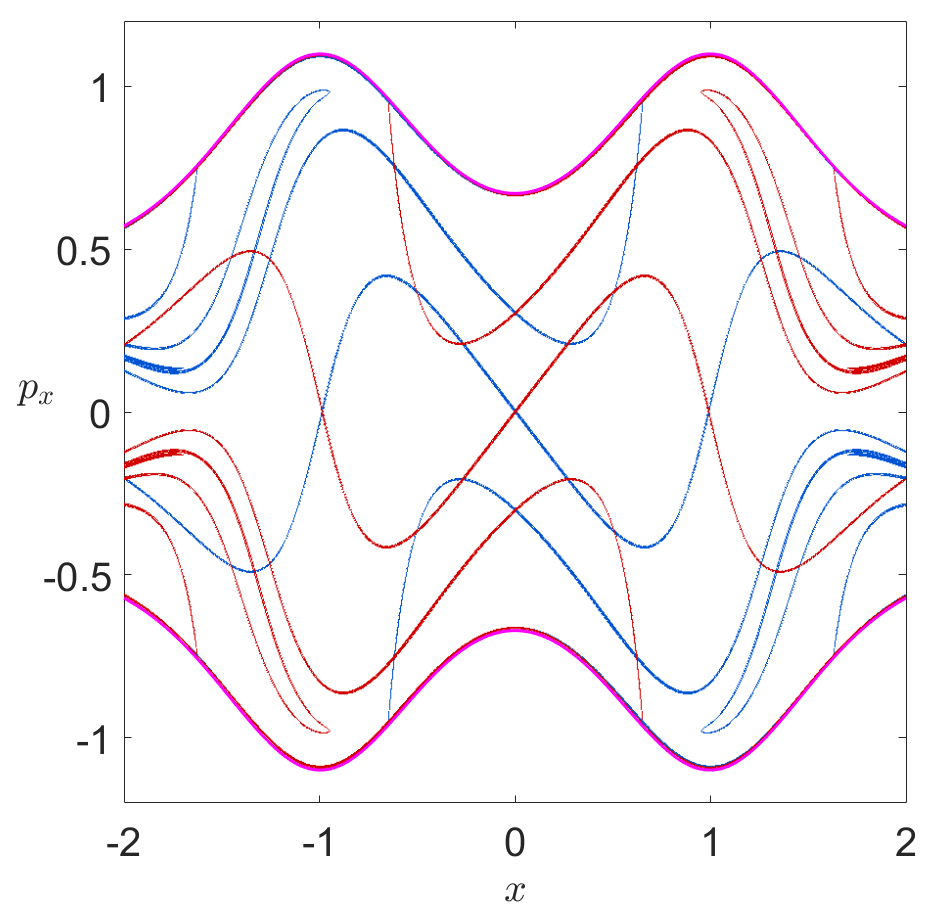
\includegraphics[scale=0.28]{H_01_mani_tau_12_y_0.png}
	\caption{Parameters $W_0 = 1/2$ and $k = 1$. Poincar\'e section $y = 0$. Top row energy $H_0 = -0.1$. Bottom row energy $H_0 = 0.1$.}
	\label{fig:ld_mani_y_0}
\end{figure}

\begin{figure}[htbp]
	A)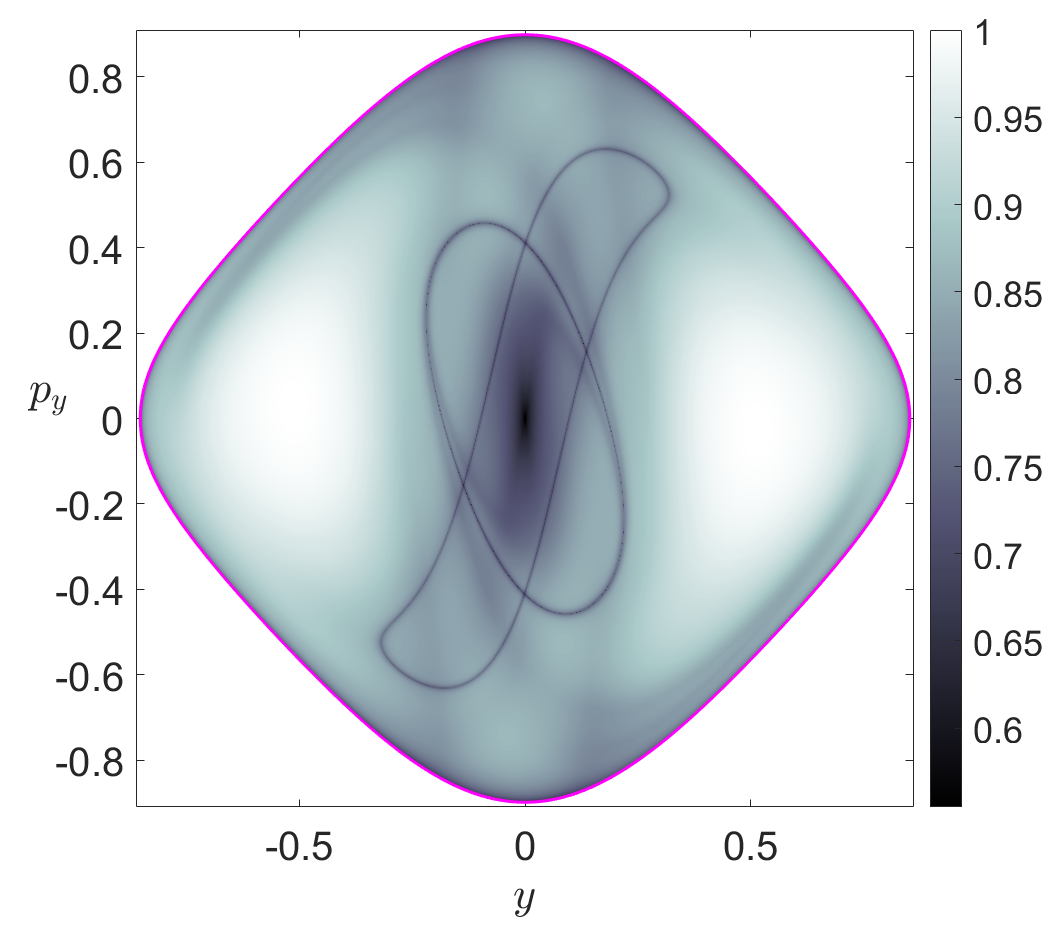
\includegraphics[scale=0.28]{H_-01_LD_tau_12_x_1.png}
	B)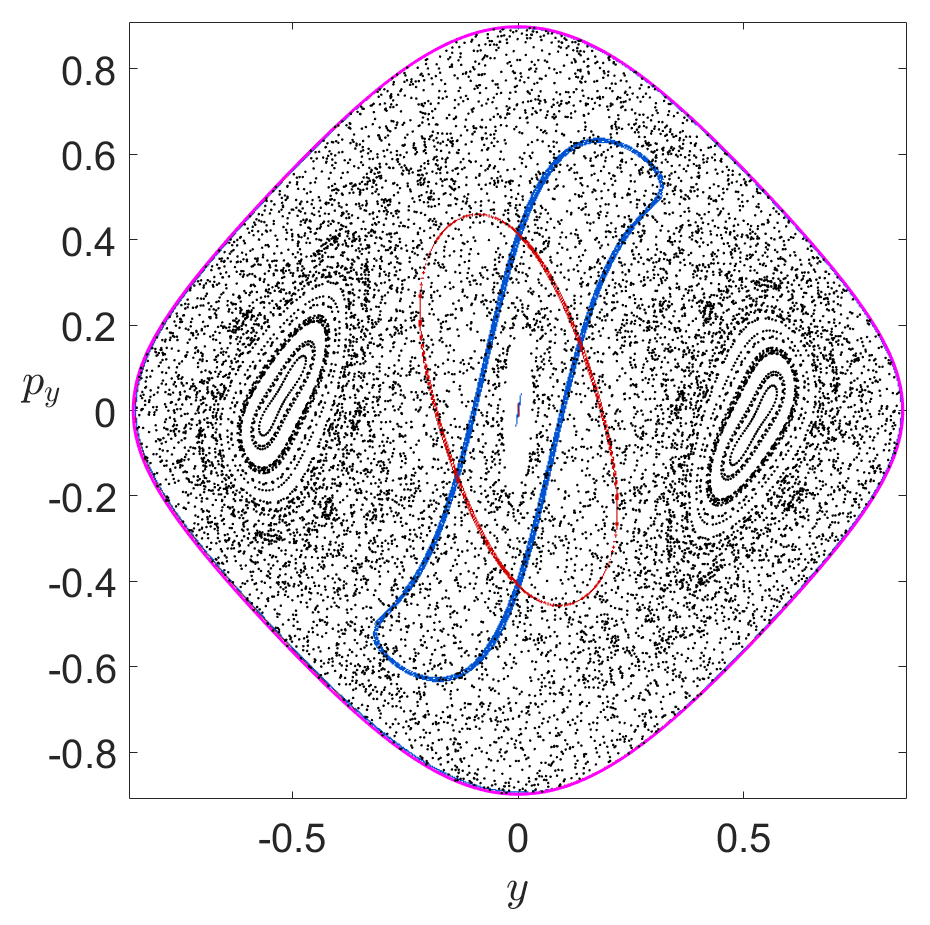
\includegraphics[scale=0.28]{H_-01_mani_tau_12_x_1.png}	
	C)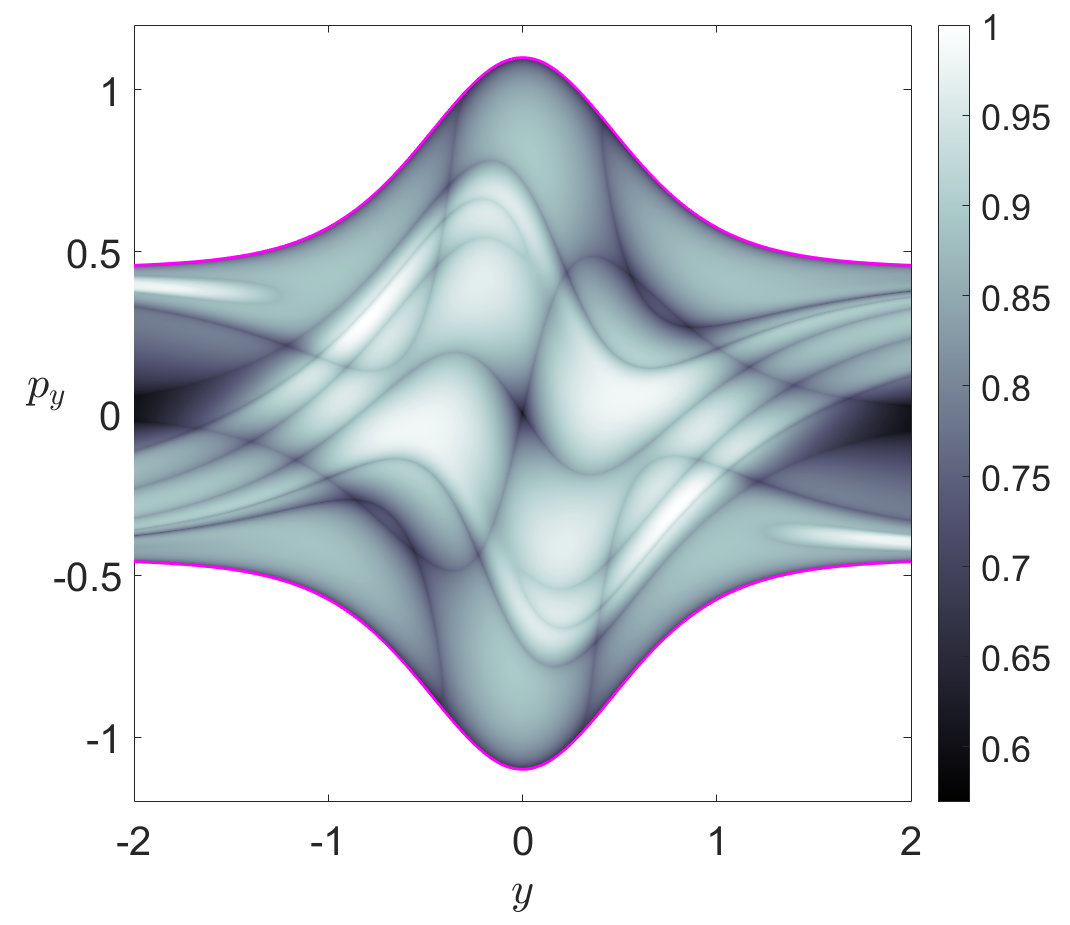
\includegraphics[scale=0.28]{H_01_LD_tau_12_x_1.png}
	D)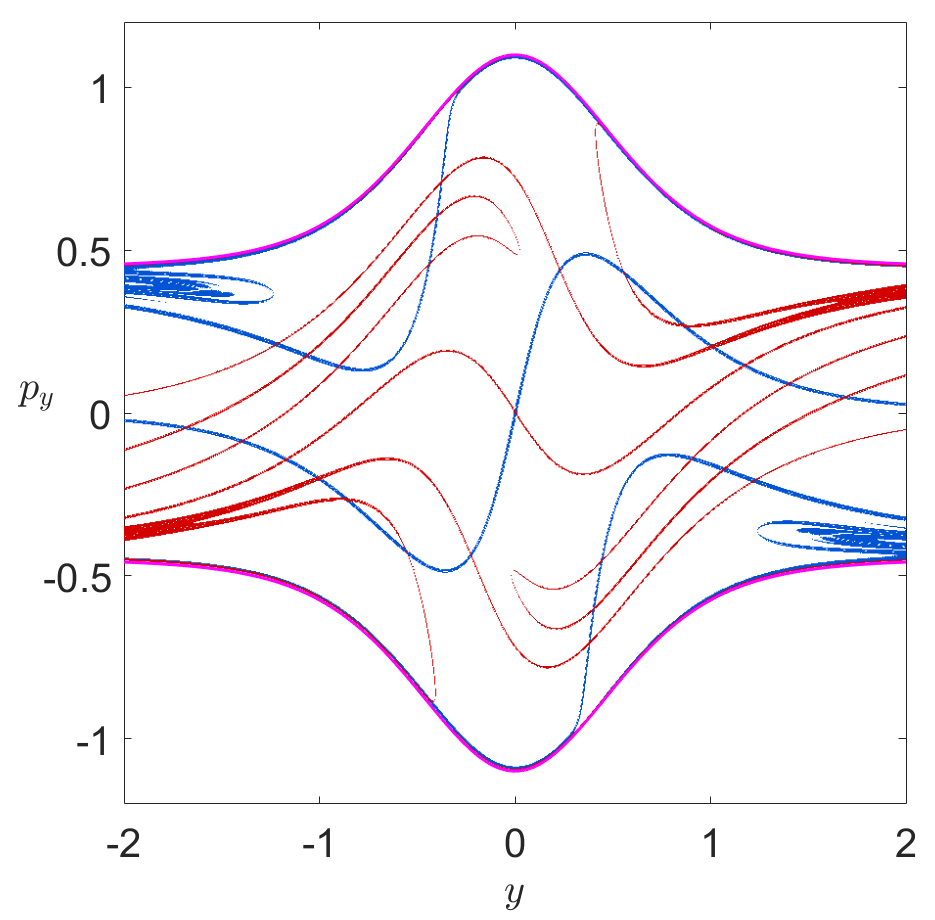
\includegraphics[scale=0.28]{H_01_mani_tau_12_x_1.png}
	\caption{Parameters $W_0 = 1/2$ and $k = 1$. Poincar\'e section $x = 1$. Top row energy $H_0 = -0.1$. Bottom row energy $H_0 = 0.1$.}
	\label{fig:ld_mani_x_1}
\end{figure}

\begin{figure}[htbp]
	A)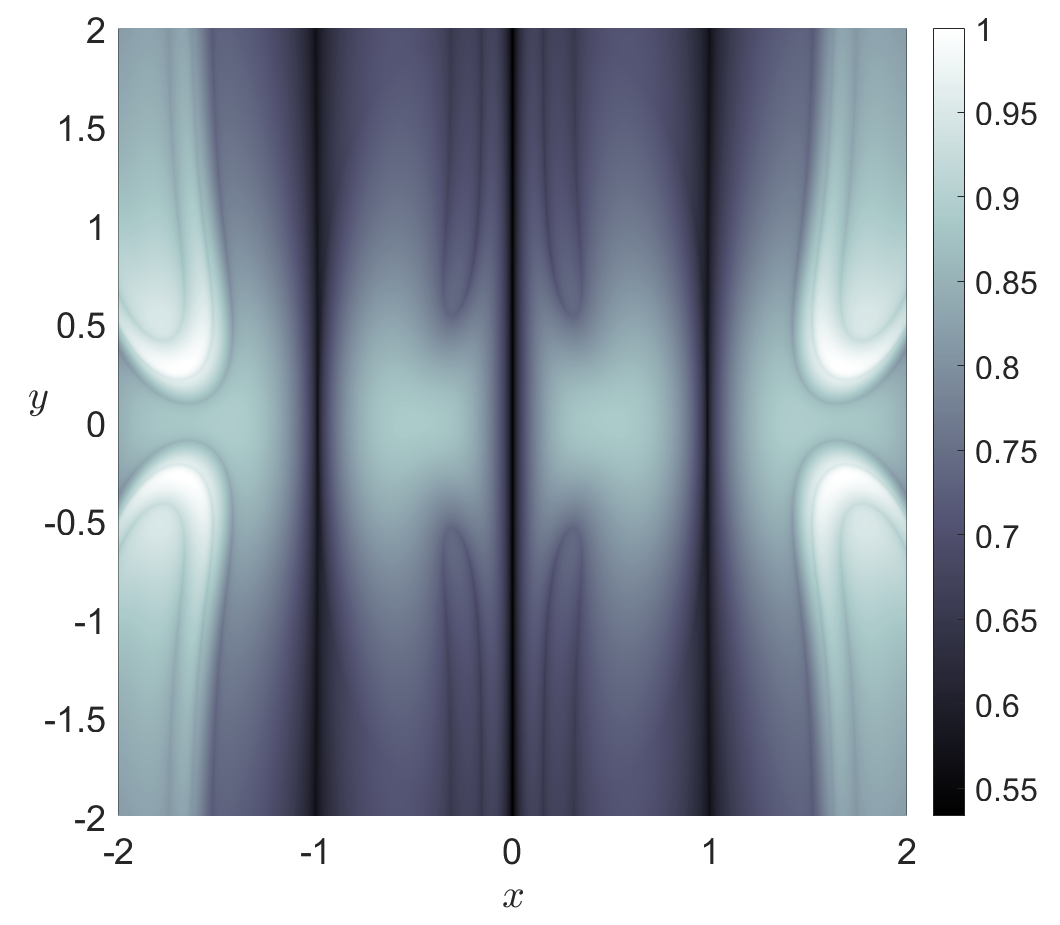
\includegraphics[scale=0.28]{H_01_LD_tau_12_px_0.png}
	B)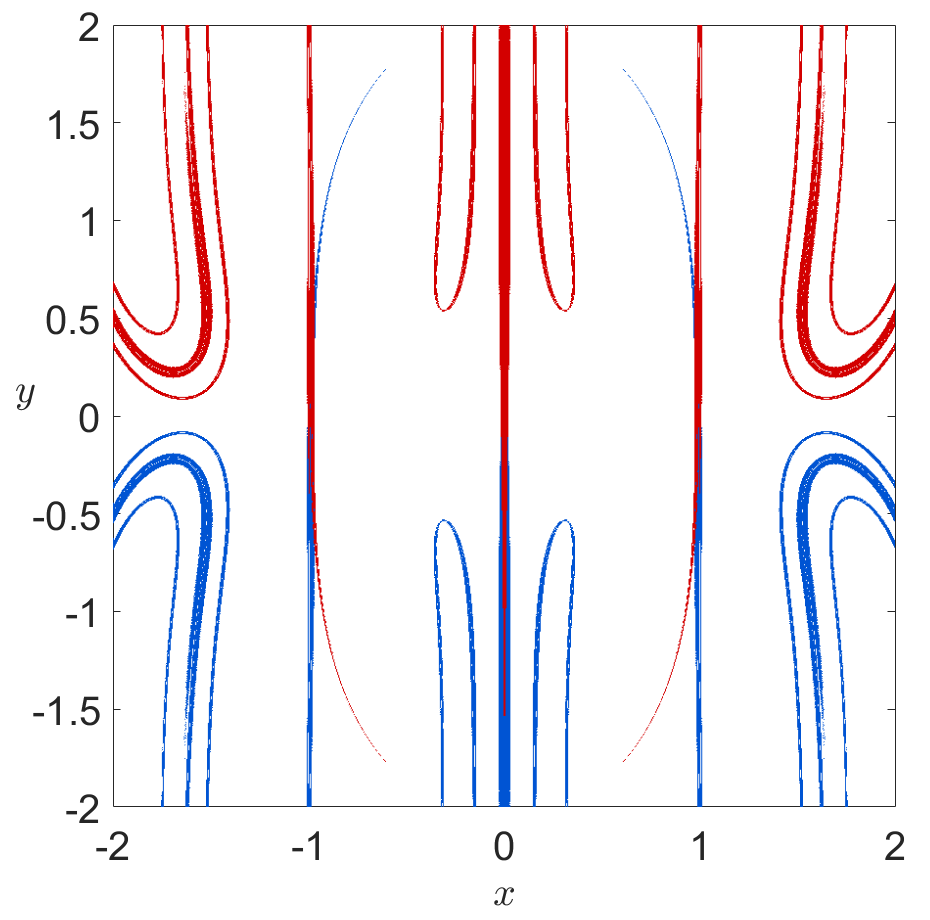
\includegraphics[scale=0.28]{H_01_mani_tau_12_px_0.png}	
	\caption{Parameters $W_0 = 1/2$ and $k = 1$. Poincar\'e section $p_x = 0$. Energy $H_0 = 0.1$.}
	\label{fig:ld_mani_px_0}
\end{figure}


\begin{figure}[htbp]
	A)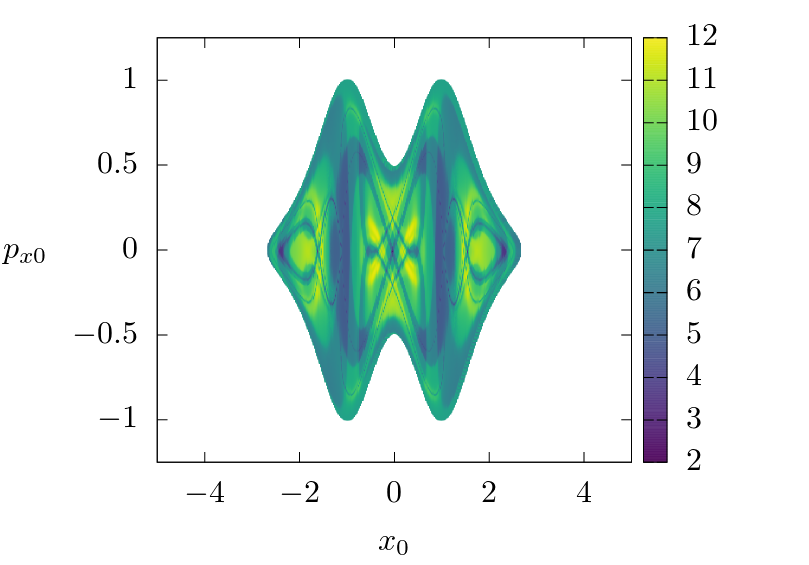
\includegraphics[scale=0.35]{ld_xpx_t20_E-001.png}
	B)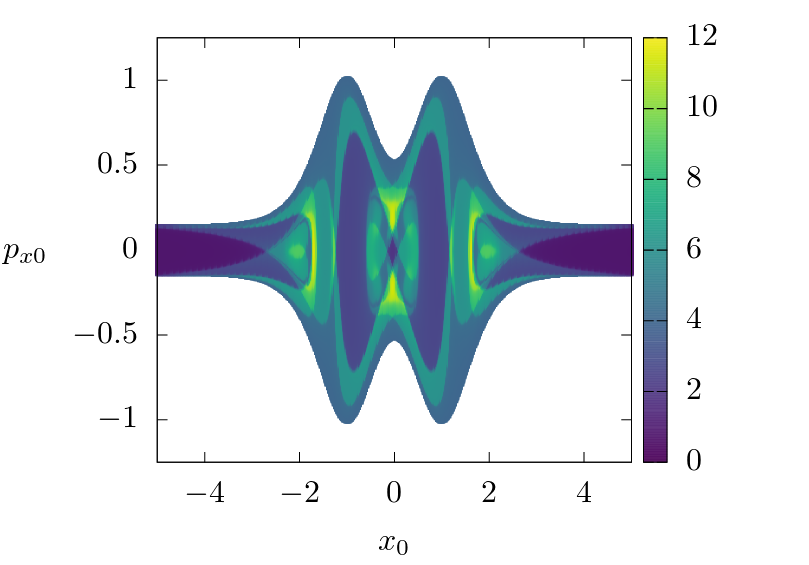
\includegraphics[scale=0.35]{ld_xpx_t20_E001.png}	
	\caption{Parameters $W_0 = 1/2$ and $k = 1$. Surface $y = 0$. $H_0 =-0.01, 0.01$.  }
	\label{fig:ld_xxxx}
\end{figure}

\begin{figure}[htbp]
	A)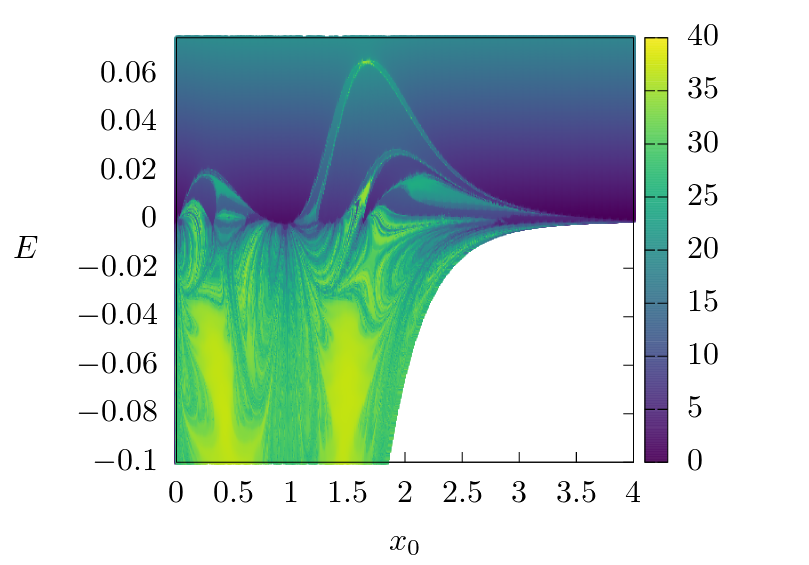
\includegraphics[scale=0.35]{ld_t60_line_x_E.png}
	B)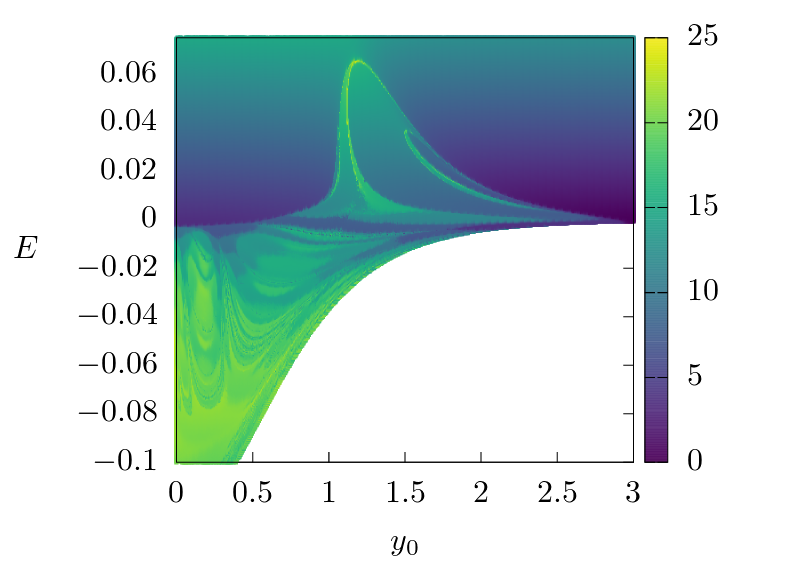
\includegraphics[scale=0.35]{ld_t60_line_y_E.png}
	\caption{ Bifurcations.  Parameters $W_0 = 1/2$ and $k = 1$. Lagrangian descriptor $E$ vs $x_0$ and $E$ vs $y_0$ }
	\label{fig:ld_E_xy}
\end{figure}

\begin{figure}[htbp]
	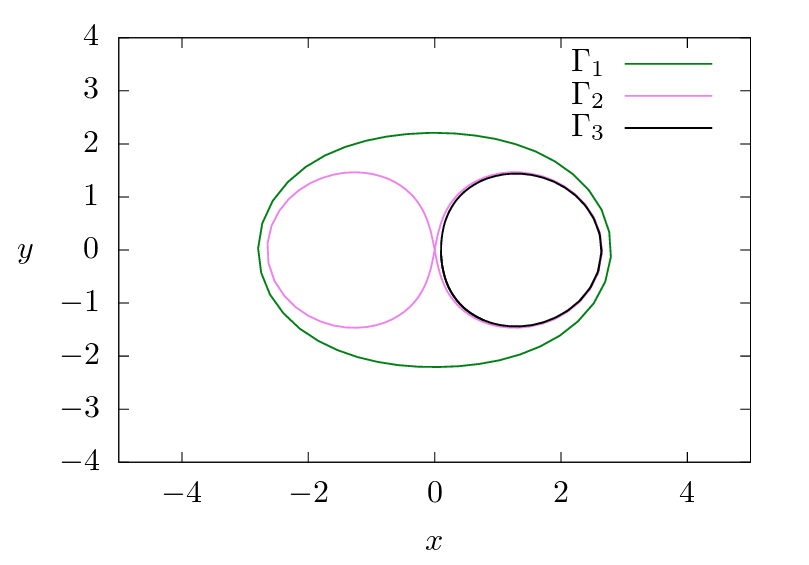
\includegraphics[scale=0.5]{orbits_2D.png}
	\caption{Periodic orbits in the configuration space. $E$ = 0.01. }
	\label{fig:ld_E_xy}
\end{figure}


\begin{figure}
    \centering
    A)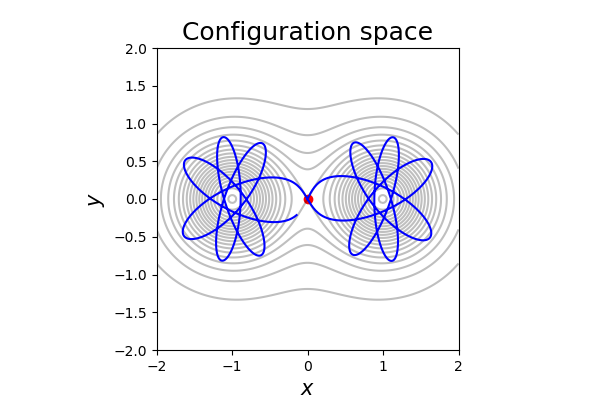
\includegraphics{traj_type2.png}
    B)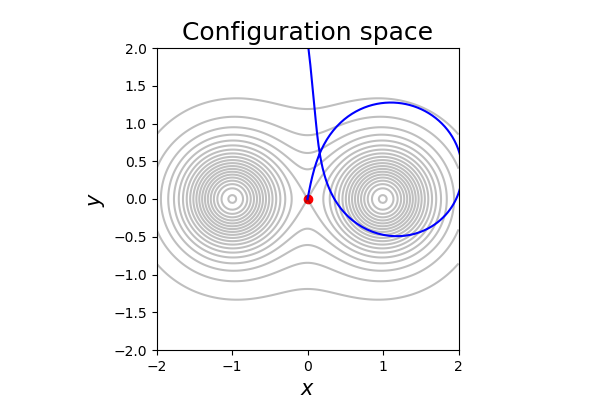
\includegraphics{traj_escapping.png}
    \caption{Example trajectories. A) $E = -0.1$, B) $E=0.01$, with identical initial condition $(x_0, y_0) = (0,0)$, and $p_{x,0} = 0.1$}
    \label{fig:my_label}
\end{figure}

\section{Conclusions}
\label{sec:conclusion}

\section*{Acknowledgments}
The authors would like to acknowledge the financial support provided by the EPSRC Grant No. EP/P021123/1 and the Office of Naval Research Grant No. N00014-01-1-0769.

\bibliography{cirque}

\end{document}
